% la-lab-07-leastsqu.tex

\documentclass[11pt]{article}
\usepackage{enumerate}
\usepackage{syllogism} 
\usepackage{october}
\usepackage[table]{xcolor}

\newcounter{aufg}
\setcounter{aufg}{0}
\newcommand{\aufgabe}[0]{\refstepcounter{aufg}\textbf{(\arabic{aufg})}}

\begin{document}

\textbf{Least Squares}

{\aufgabe} Consider the following function:
\begin{equation}
f\left(\left[
\begin{array}{c}
x \\
y
\end{array}\right]\right)=\left[
\begin{array}{c}
x^{2}+x\sin(x+y) \\
\sin{}x\cos(x+y)
\end{array}\right]\notag
\end{equation}
Linearize the function around $x=\frac{\pi}{2},y=\frac{\pi}{2}$ so it looks as follows,
\begin{equation}
  f(x)\approx{}\left[
    \begin{array}{c}
      P \\
      Q
    \end{array}\right]
+\left[
\begin{array}{cc}
A&B \\
C&D
\end{array}\right]\left[
\begin{array}{c}
x-M \\
y-N
\end{array}\right]\notag
\end{equation}
Specify the numbers $A,B,C,D,,M,N,P,Q$ in your solution.

{\aufgabe} Project the vector $y=(4,-6,-10,-10)^{\intercal}$ onto the
plane containing the points
\begin{equation}
  \label{eq:eareisoo}
  P=(-7,8,3,0),Q=(-3,11,2,6),R=(-4,11,12,-2)\notag
\end{equation}

{\aufgabe} Project the vector $y=(4,-6,-10,-10)^{\intercal}$ onto the
plane containing the points
\begin{equation}
  \label{eq:aecathie}
  P=(-7,8,3,0),Q=(-3,11,2,6),R=(-2,11,-8,14)\notag
\end{equation}
You should get the same answer as in the last question, but your
procedure will probably be different.

{\aufgabe} At 6327 ft (or 6.327 thousand feet), Mario Triola recorded
  the temperature. Find the best predicted temperature at that
  altitude based on other measurements, assuming a linear
  relationship. How does the result compare to the actual recorded
  value of 48$^{\circ}$F?

\begin{tabular}{|l|l|l|l|l|l|l|l|}
\hline
Altitude (in thousand ft) & 3 & 10 & 14 & 22 & 28 & 31 & 33 \\
\hline
Temperature & 57 & 37 & 24 & -5 & -30 & -41 & -54 \\
\hline
\end{tabular}

Do this both ways, using the $Y-AV=E$ setup and projection on the one
hand and, on the other hand, the formula
\begin{equation}
  \label{eq:iduochuk}
    V_{0}=\left[
      \begin{array}{c}
        m \\
        b
      \end{array}\right]=(A^{\intercal}A)^{-1}A^{\intercal}Y  \notag
\end{equation}

{\aufgabe} You measure the four angles in a quadrilateral
$\hat{a}=8.490426^{\circ},\hat{b}=182.029154^{\circ},\hat{c}=119.148088^{\circ},\hat{d}=50.32948$.
What are the least squares adjusted measurements?

{\aufgabe} Consider the following leveling network. 
    \begin{figure}[h]
    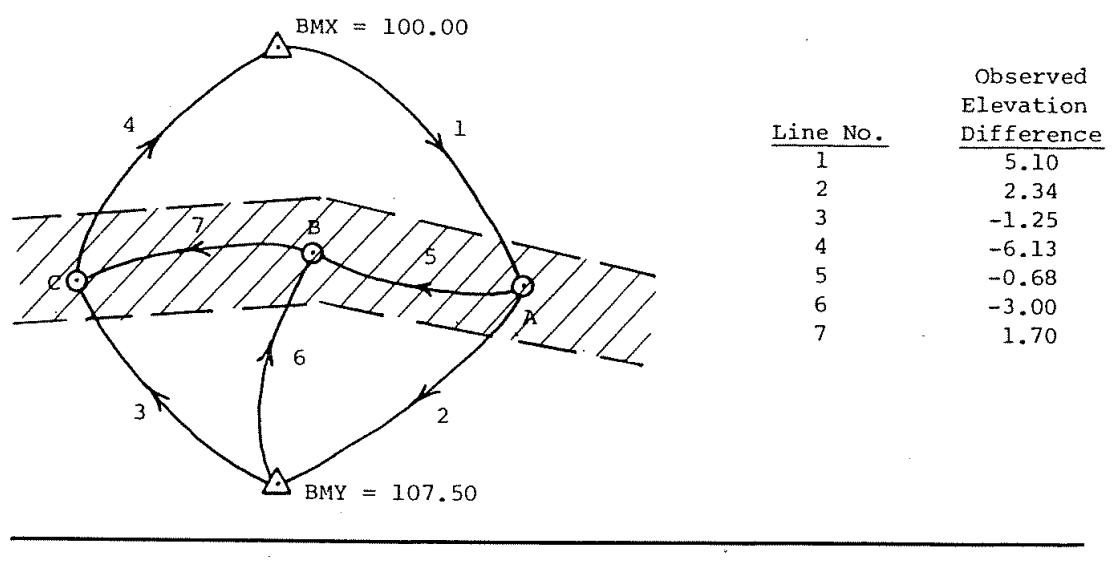
\includegraphics[scale=0.26]{./diagrams/levelingnetwork.png}
  \end{figure}
  The objective is to determine elevations of $A$, $B$, and $C$, which
  are to serve as temporary project bench marks to control
  construction of a highway through the crosshatched corridor.

Calculate the least squares
  adjusted elevations of $A$, $B$, and $C$ using the following
  observation equations.
  \begin{equation}
    \label{eq:aelaeghu}
    \begin{array}{rcl}
      A&=&BMX+5.10+\epsilon_{1} \\
      BMY&=&A+2.34+\epsilon_{2} \\
      C&=&BMY-1.25+\epsilon_{3} \\
      BMX&=&C-6.13+\epsilon_{4} \\
      B&=&A-0.68+\epsilon_{5} \\
      B&=&BMY-3.00+\epsilon_{6} \\
      C&=&B+1.70+\epsilon_{7}
    \end{array}\notag
  \end{equation}

{\aufgabe} Calculate the distance between the vector
$\vec{v}=(-6,5,5,-2)^{\intercal}$ and the hyperplane
\begin{equation}
  \label{eq:eixaekaw}
  \left\{\left.\vec{x}\in\mathbb{R}^{4}\;\right\vert\;\vec{x}=s_{1}\left(
      \begin{array}{c}
        3 \\
        -9 \\
        -10 \\
        3
      \end{array}\right)+s_{2}\left(
      \begin{array}{c}
        3 \\
        0 \\
        -8 \\
        -9
      \end{array}\right)+s_{3}\left(
      \begin{array}{c}
        1 \\
        6 \\
        8 \\
        -9
      \end{array}\right)\right\}\notag
\end{equation}

\end{document}
